\chapterWithSubtitle{Context-Free Languages and Turing Machines}{February 18, 2021}

\section{Context Free Languages}

\subsection{Context Free Languages}
\begin{itemize}
    \item[] 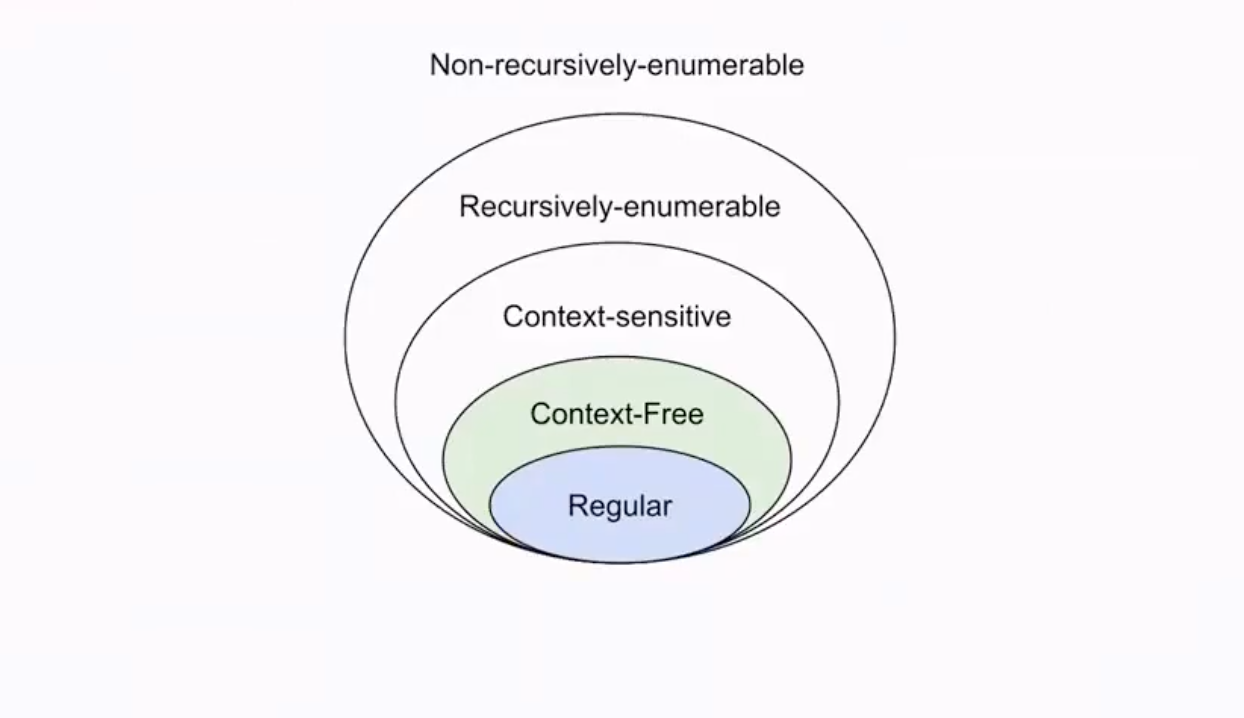
\includegraphics[width=\textwidth]{lecture8/images/chomsky-hierarchy-context-free.png}
    \item Example (Palindrome):
    \begin{itemize}
        \item $V = \{ S \}$
        \item $T = \{ a, b \}$
        \item $P = \{ S \rightarrow \epsilon \mid a \mid b \mid aSa \mid bSb \}$. $P$ is complete, so $P$ must go to $\epsilon$ or one of the terminal symbols ($a$ or $b$).
    \end{itemize}
    \item \textbf{Context Free Languages} includes any string that can be derived from these production rules.
\end{itemize}

\subsection{Context Free Grammar}
\begin{itemize}
    \item A \textbf{Context Free Grammar (CFG)} is a quadruple $G = (V, T, P, S)$:
    \begin{itemize}
        \item $V$ is a finite set of \textbf{non-terminal symbols} (variables).
        \item $T$ is a finite set of \textbf{terminal symbols} (alphabet).
        \item $P$ is a finite set of \textbf{productions}, each of the from $A \rightarrow \alpha$ where $A \in V$ and $\alpha$ is a string in $(V \cup T)^{\ast}$. Formally, $P \subset V \times (V \cup T)^{\ast}$.
        \item $S \in V$ is a \textbf{start symbol}.
    \end{itemize}
    \item The language generated by CFG $G = (V, T, P, S)$ is denoted by $L(G)$ where $L(G) = \{ w \in T^{\ast} \mid S \leadsto^{\ast} w \}$.
    \item A language $L$ is \textbf{context free (CFL)} if it is generated by a context free grammar. That is, there is a CFG $G$ such that $L = L(G)$.
\end{itemize}

\section{Context Sensitive Languages}

\subsection{Context Sensitive Languages}
\begin{itemize}
    \item[] 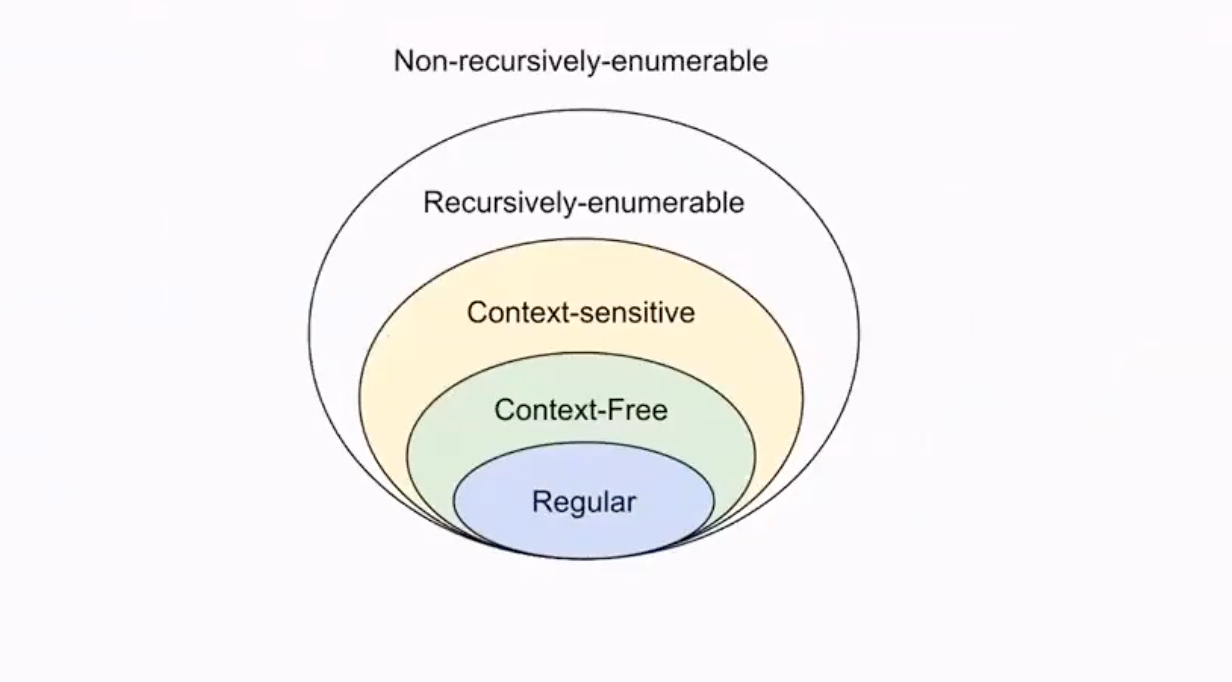
\includegraphics[width=\textwidth]{lecture8/images/chomsky-hierarchy-context-sensitive.png}
    \item The language $L = \{ a^n b^n c^n \mid n \geq 1 \}$ is not a context free language, and can be proved via the \textbf{pumping lemma}:
    \begin{itemize}
        \item $V = \{ S, A, B \}$
        \item $T = \{ a, b, c \}$
        \item $P = \left\{
            \begin{tabular}{c}
                $S \rightarrow abc \mid aAbc$ \\
                $Ab \rightarrow bA$ \\
                $Ac \rightarrow Bbcc$ \\
                $bB \rightarrow Bb$ \\
                $aB \rightarrow aa \mid aaA$
            \end{tabular}
        \right\}$
    \end{itemize}
\end{itemize}

\subsection{Context Sensitive Grammar}
\begin{itemize}
    \item A \textbf{Context Sensitive Grammar (CSG)} is a quadruple $G = (V, T, P, S)$:
    \begin{itemize}
        \item $V$ is a finite set of \textbf{non-terminal symbols}.
        \item $T$ is a finite set of \textbf{terminal symbols}.
        \item $P$ is a finite set of \textbf{productions}, each of the form $\alpha \rightarrow \beta$ where $\alpha$ and $\beta$ are string in $(V \cup T)^{\ast}$.
        \item $S \in V$ is a \textbf{start symbol}.
    \end{itemize}
\end{itemize}

\section{Turing Machines}

\subsection{"Most General" Computer}
\begin{itemize}
    \item DFAs are a simple model of computation and only accept the regular languages.
    \item The idea behind a Turing Machine is to create a computer that can accept any language, or compute any function.
    \item Counting argument: the set of all languages is $\{ L \mid L \subseteq \{ 0, 1 \}^{\ast} \}$ (uncountably infinite).
    \item The set of all programs is $\{ P \mid P \text{ is a finite length computer program} \}$ is countably infinite.
    \item \textit{Conclusion}: There are languages for which there are no programs.
    \item Onto recursively enumerable languages.
    \item[] 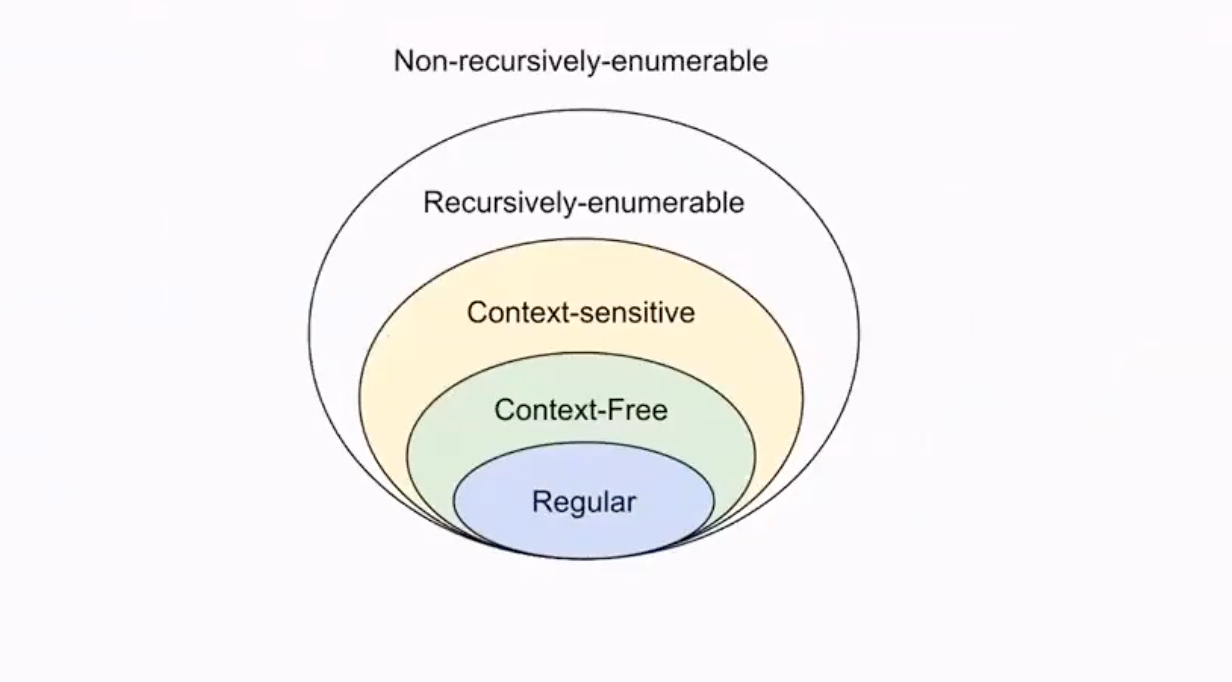
\includegraphics[width=\textwidth]{lecture8/images/chomsky-hierarchy-context-sensitive.png}
\end{itemize}

\subsection{What is a Turing Machine?}
\begin{itemize}
    \item Input written on (infinite) one sided tape
    \item Special blank characters
    \item Finite state control (similar to DFA)
    \item Every step: Read character under head, write character out, move the head right of left (or stay).
\end{itemize}

\subsection{High Level Goals}
\begin{itemize}
    \item Church-Turing thesis: TMs are the most general computing devices. So far, no counter example.
    \item Every TM can be represented as a string.
    \item Existence of \textbf{Universal Turing Machine}, which is the model/inspiration for stored program computing. UTM can simulate any TM.
    \item Implications for what can be computed and what cannot be computed.
\end{itemize}

\subsection{Turing Machine Formal Definition}
\begin{itemize}
    \item A \textbf{Turing Machine} is a 7 tuple $(Q, \sum, \Gamma, \delta, q_0, q_{\text{acc}}, q_{\text{rej}})$:
    \item $Q$: finite set of states
    \item $\sum$: finite input alphabet
    \item $\Gamma$: finite tape alphabet (includes $\textvisiblespace$ and $:$)
    \item $\delta: Q \times \Gamma \rightarrow Q \times \Gamma \times \{ L, S, R \}$: transition function
    \item $q_0 \in Q$: the initial state
    \item $q_{\text{acc}} \in Q$: the accepting/final state
    \item $q_{\text{rej}} \in Q$: the rejecting state
\end{itemize}

\subsection{Turing Machine: Transition Function}
\begin{itemize}
    \item $\delta: Q \times \Gamma \rightarrow Q \times \Gamma \times \{ L, R, S \}$
    \item As such, the transition $\delta(q, c) = (p, d, L)$
    \item[] 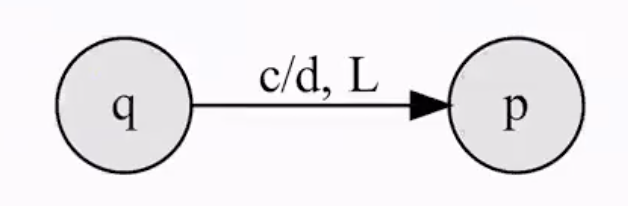
\includegraphics[width=0.6\linewidth]{lecture8/images/turing-transition-function.png}
    \item $q$: current state
    \item $c$: character under tape head
    \item $p$: new state
    \item $d$: character to write under tape head
    \item $L$: move tape head left
    \item Missing transitions lead to hell state: "Blue screen of death" or "Machine crashes"
\end{itemize}

\subsection{Languages Defined by Turing Machines}
\begin{itemize}
    \item Recursively enumerable (aka RE) languages
    \begin{equation}
        L = \{ L(M) \mid M \text{ some Turing machine} \}
    \end{equation}
    \item Recursively/decidable languages
    \begin{equation}
        L = \{ L(M) \mid M \text{ some Turing machine that halts on all inputs} \}
    \end{equation}
\end{itemize}
